\documentclass{article}

\usepackage{titlesec}
\titlelabel{\thetitle.\quad}

\usepackage[T1]{fontenc}
\usepackage{inconsolata}

\usepackage[english]{babel}
\usepackage[letterpaper,top=2cm,bottom=2cm,left=2cm,right=2cm,marginparwidth=1.25cm]{geometry}

\usepackage{hyperref, booktabs, float}
\usepackage[leqno]{amsmath}
\usepackage{enumitem, nccmath,lipsum,amssymb,xcolor,xparse,listings, blindtext}
\usepackage[most]{tcolorbox}

\setlength{\parindent}{6pt}

\definecolor{codegreen}{rgb}{0,0.6,0}
\definecolor{codegray}{rgb}{0.5,0.5,0.5}
\definecolor{codepurple}{rgb}{0.58,0,0.82}
\definecolor{backcolour}{rgb}{0.95,0.95,0.92}

\lstdefinestyle{mystyle}{
    backgroundcolor=\color{backcolour},   
    commentstyle=\color{codegreen},
    keywordstyle=\color{magenta},
    numberstyle=\tiny\color{codegray},
    stringstyle=\color{codepurple},
    basicstyle=\ttfamily\footnotesize,
    breakatwhitespace=false,         
    breaklines=true,                 
    captionpos=b,                    
    keepspaces=true,                 
    numbers=left,                    
    numbersep=5pt,                  
    showspaces=false,                
    showstringspaces=false,
    showtabs=false,                  
    tabsize=2
}

\lstset{style=mystyle}

\usepackage{graphicx}
\graphicspath{ {./attachments/} }

\definecolor{light-gray}{gray}{0.9}
\newcommand{\code}[1]{\colorbox{light-gray}{\texttt{#1}}}

\title{Indexes In Relational Databases}
\author{Mashenkov Timofei \\ \href{t.me/mashfeii}{mashfeii}}
\begin{document}
\maketitle{}

\section{Introduction}

Index is a special object which is created for single or several columns. It is used to speed up the search of data in the table. It can be compared with book and its table of contents, where you can find the necessary information much faster than just reading the book from the beginning to the end.

\subsection{Simple Example}
\noindent

\begin{lstlisting}[language=SQL, caption={Simple example of table creation}]
CREATE TABLE users (
    id INT PRIMARY KEY,
    first_name VARCHAR(255),
    last_name VARCHAR(255),
    city VARCHAR(255),
);
\end{lstlisting}

If we fill the following table with 1 million records and try to retrieve all users from Moscow city, the query will take a long time: \newline

\code{EXPLAIN ANALYZE SELECT * FROM users WHERE city = 'Moscow';} \newline

Such query can take up to 180ms of execution time, so we need to optimize it: \newline

\code{CREATE INDEX idx\_users\_city\_hash ON users USING HASH (city);} \newline

Such adjustment will reduce execution time to 30ms in average, also the Scan type will be changed to Index Scan.

\section{Types of Indexes}

\begin{itemize}
  \item \textbf{B-Tree} - the most common type of index. It is used for columns with low cardinality.
  \item \textbf{Hash} - used for columns with high cardinality.
  \item \textbf{GiST} - used for geometric data types.
  \item \textbf{GIN} - used for indexing array data types.
  \item \textbf{BRIN} - used for very large tables.
\end{itemize}

\subsection{Partial Index}
\noindent

Index may be created only for the \textbf{subset of data}, not the whole table. It is useful when you need to index only a part of the table.

\begin{lstlisting}[language=SQL, caption={Partial index example}]
  CREATE INDEX idx_users_city_moscow ON users (email) WHERE city = 'Moscow';
\end{lstlisting}

\subsection{B-Tree}
\noindent

\begin{itemize}
  \item Universal index for most cases (\code{=}, \code{<}, \code{>}, \code{<=}, \code{>=}, \code{BETWEEN}, \code{ORDER BY}).
  \item Used in \code{PRIMARY KEY}, \code{UNIQUE}, \code{FOREIGN KEY} constraints and within filtering on equality (\code{WHERE column = 'value'}).
  \item Does not fit the full-text search (\code{LIKE '\%text\%'}).
  \item Can slow down inserting and updating.
\end{itemize}

\subsection{Hash}
\noindent

\begin{itemize}
  \item Fast and concise, but only for \code{=} operator.
  \item Not used for ranges (\code{<}, \code{>}, \code{BETWEEN}) and sorting (\code{ORDER BY}).
  \item In PostgreSQL works better on fields like \code{user\_id}, \code{email}, \code{ip\_address}.
  \item \textbf{If you are not sure, use \code{B-Tree}}. 
\end{itemize}

\subsection{GiST}
\noindent 

\begin{itemize}
  \item Universal index for complex data types 
  \item Used for geodata, ranges, arrays, \code{JSONB}, full-text search.
  \item Does not replace B-Tree for \code{=}, \code{BETWEEN}, \code{ORDER BY}.
  \item Alternatives: for text (\code{GIN}), for standard requests (\code{B-Tree}).
\end{itemize}

\subsection{GIN}
\noindent

\begin{itemize}
  \item The best fit for the \code{JSONB}, arrays, full-text search.
  \item Works faster than \code{B-Tree}, \code{GiST} for searching complex data types.
  \item Slow under the \code{INSERT}/\code{UPDATE}/\code{DELETE} operations, does not support \code{ORDER BY}.
\end{itemize}

\subsection{BRIN}
\noindent

\begin{itemize}
  \item The best fit for very large tables with ordered data.
  \item Occupies much less space and speed up range requests.
  \item Does not replace \code{B-Tree}, but perfectly works with time data.
  \item \textbf{If the data is not ordered, \code{BRIN} is useless}. 
\end{itemize}

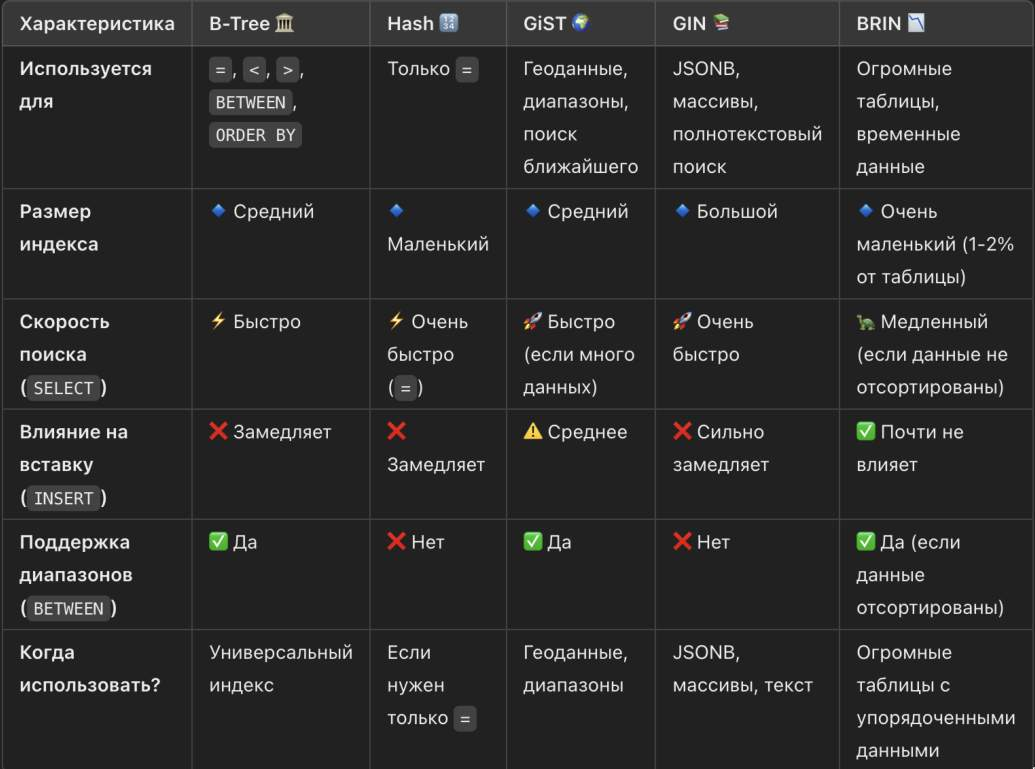
\includegraphics[width=\textwidth]{../attachments/indexes.jpg}

\section{PostgreSQL Optimizations}

Request within the time of execution also contains the time of planning. Planning stands for the time when Database Management System (DBMS) decides how to execute the query.

\begin{table}[H]
  \centering
  \begin{tabular}{|c|c|}
    \toprule
    Type of Optimization & What is does? \\ \midrule
    Rewriting Rules & Simplifies \code{WHERE}, \code{IN}, \code{JOIN}, \code{CTE} \\ \midrule
    Indexes Using & \code{Index Scan}, \code{Index Only Scan}, \code{Bitmap Index Scan} \\ \midrule
    \code{JOIN} Optimization & \code{Nested Loop}, \code{Hash Join}, \code{Merge Join} \\ \midrule 
    \code{ORDER BY} Optimization & Using indexes instead of sorting \\ \midrule 
    Parallel Execution & Parallels \code{SELECT}, \code{JOIN}, \code{AGGREGATE} \\
    \bottomrule
  \end{tabular}
  \caption{PostgreSQL Optimizations}
\end{table}


\end{document}
